\chapter{Experiments in RGBD sensing using DepthAI} \label{experiments_oak_d}

\section{Overview}

%In this chapter, we present the design and implementation of our solution, focusing on visual mapping and 3D reconstruction. The experiments and methodologies employed in this thesis aim to evaluate the performance and capabilities of various tools and techniques for real-time mapping and object detection.

In this chapter we explore the capabilities of the OAK-D camera using the DepthAI Viewer software to understand its functionalities. This exploration provided insights into the camera's real-time 3D reconstruction and its Vision Processing Unit (VPU) capabilities. Subsequently, we experimented with the Spectacular AI SDK to further test the camera's performance, especially in mapping and person detection scenarios.

%%% Overall, this chapter provides a comprehensive overview of the experimental design, methodologies, and outcomes of our efforts to develop an effective solution for real-time mapping and 3D reconstruction using state-of-the-art technologies.

\section{DepthAI Viewer}

To begin exploring the capabilities of the camera, I initiated my efforts by testing the example software provided by the camera's manufacturer, namely DepthAI Viewer\footnote{\url{https://github.com/luxonis/depthai-viewer}}. This software proved invaluable for its ability to showcase the camera's functionalities effectively.

Upon installation, I gained access to a user-friendly interface that allowed me to view images captured by the camera in real time. Additionally, the software facilitated real-time 3D reconstruction of the camera's surroundings, as depicted in Figure~\ref{fig:DAI_3d}. Notably, the DepthAI Viewer leveraged the Vision Processing Unit (VPU) embedded within the device, thereby enabling comprehensive exploration of its capabilities, as illustrated in the top left corner of Figure~\ref{fig:DAI_person_detection}.

\begin{figure}[htbp]
	\centering
	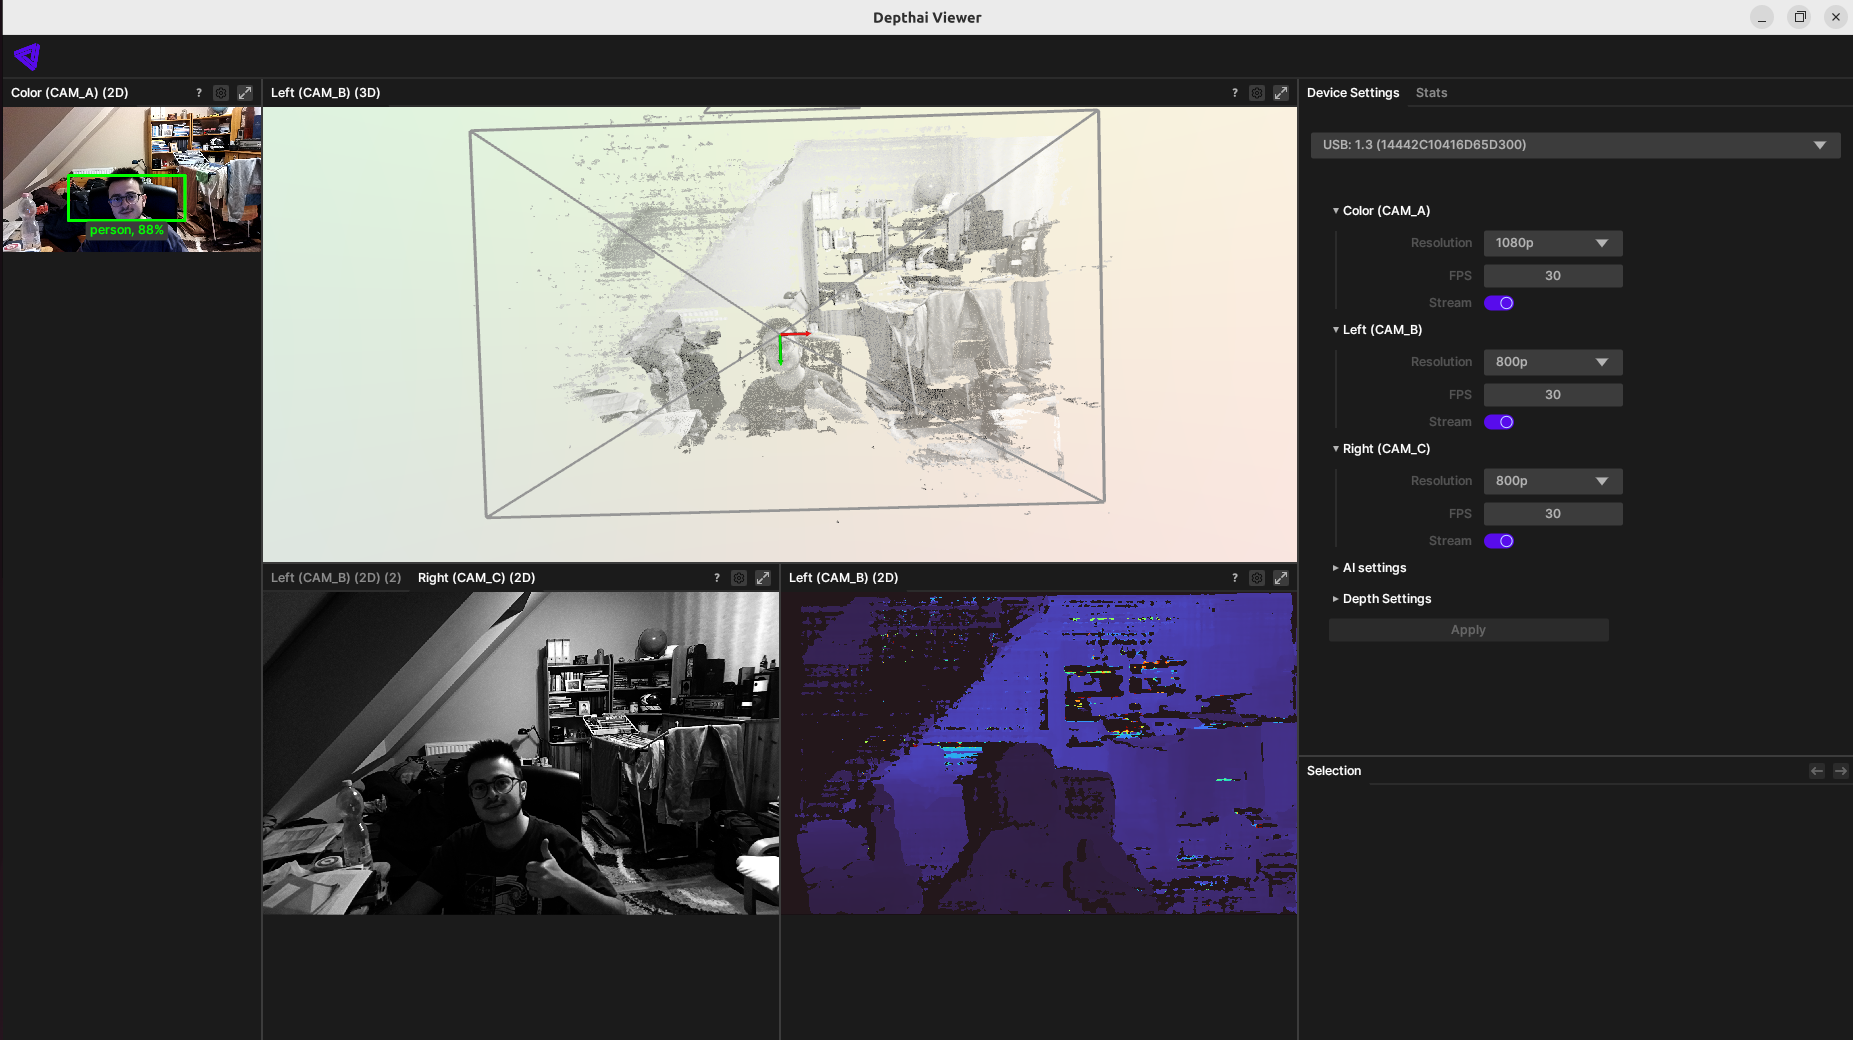
\includegraphics[width=150mm, keepaspectratio]{figures/depthai_viewer.png}
	\caption{DepthAI Viewer with person detection}
	\label{fig:DAI_person_detection}
\end{figure}

\begin{figure}[htbp]
	\centering
	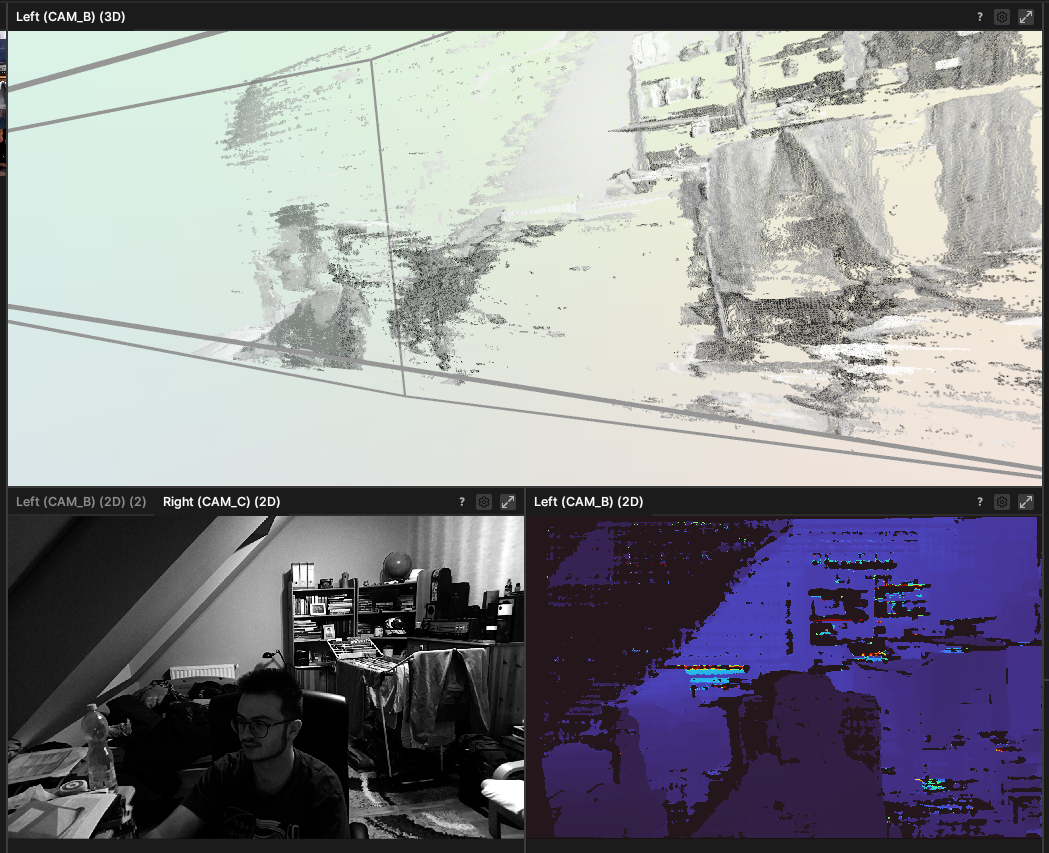
\includegraphics[width=150mm, keepaspectratio]{figures/depthai_viewer_3d.png}
	\caption{DepthAI Viewer's 3D reconstruction}
	\label{fig:DAI_3d}
\end{figure}

This initial exploration served as a foundational step in understanding the camera's capabilities and paved the way for further experimentation and development in subsequent tasks.


\section{Experimenting with Spectacular AI} \label{experiments_spai}

The next step was to experiment with the Spectacular AI SDK's examples to determine if it is capable of mapping and detecting persons with low latency. At first the Python scripts threw a warning and they did not work: 
\FloatBarrier
\begin{lstlisting}[language=bash,frame=single,float=h]
SpectacularAI WARN: Dropping frames!
SpectacularAI WARN: VIO may be running too slow, data is being input too fast, or IMU samples are missing / time-offset from frames. (buffer size 10)
\end{lstlisting}
After some research, I found out that this problem is related to outdated firmware version on the camera (note that it took a long time to find the solution due to the severe lack of documentation). To solve the issue, Luxonis' \verb|depthai-python| repo\footnote{\url{https://github.com/luxonis/depthai-python}} must be cloned and the IMU firmware update script\footnote{\url{https://github.com/luxonis/depthai-python/blob/main/examples/IMU/imu_firmware_update.py}} must be ran. After the successful firmware update I was able to try out the examples.

The simplest example is the one that visualizes the camera's movement. It extracts the data from the IMU and uses matplotlib for visualization. As we can see on Figure \ref{fig:IMU_visu}, I was able to draw a heart in the air. The curves are not perfect because my hand was probably shaking a bit.

\begin{figure}[htbp]
	\centering
	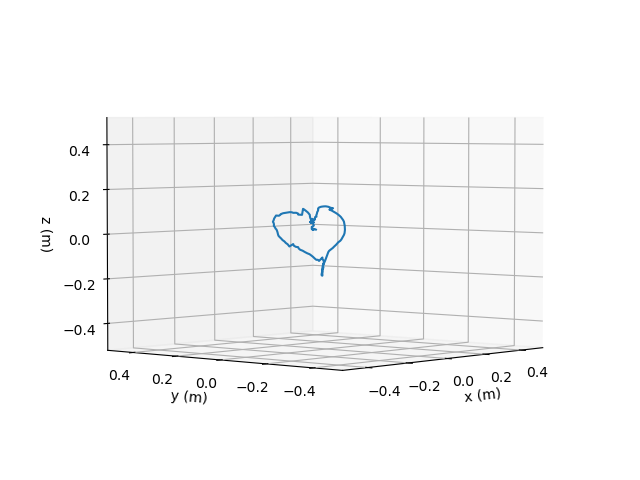
\includegraphics[width=150mm, keepaspectratio]{figures/spectacular_ai_vio_visu.png}
	\caption{IMU visualization with Spectacular AI}
	\label{fig:IMU_visu}
\end{figure}

A bit more advanced example uses the camera too, not just the IMU. When the camera is covered with our hand it visualizes the device's movement with the help of the IMU as we can see on Figure \ref{fig:3d_pen}.

\begin{figure}[htbp]
	\centering
	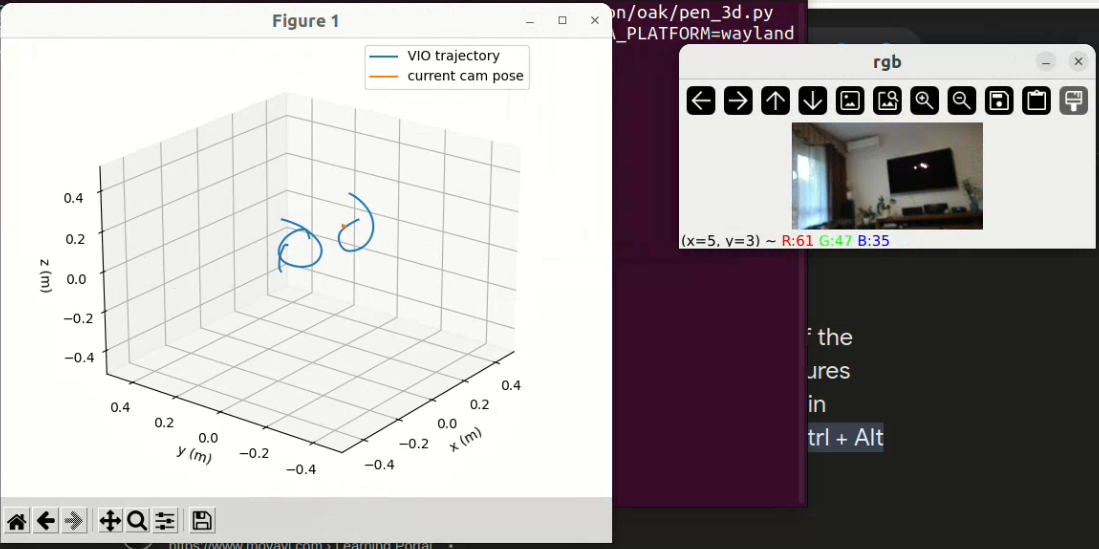
\includegraphics[width=150mm, keepaspectratio]{figures/3d_pen.png}
	\caption{IMU visualization with Spectacular AI}
	\label{fig:3d_pen}
\end{figure}

These examples just visualized the camera's movement and the picture taken with the camera so we did not see any mapping or person detection yet. The repository fortunately provides some spectacular examples on these applications too. However these examples always raised an error which had to be debugged. These examples use OpenGL for visualization and the problem stood in some deep OpenGL code. The easiest way to solve this problem was to comment out some code in \verb|OpenGL/contexdata.py|:

\begin{lstlisting}[language=python,frame=single,float=!ht]
def getContext( context = None ):
    """Get the context (if passed, just return)
    context -- the context ID, if None, the current context
    """
    if context is None:
        context = platform.GetCurrentContext()
    # if context == 0:
        # from OpenGL import errorS
        # raise error.Error(
        # """Attempt to retrieve context when no valid context"""
        # )
    return context
\end{lstlisting}
\FloatBarrier

We can try out some mapping applications, such as point cloud mapping (Figure~\ref{fig:SPAI_mapping}), real-time AR mapping with mesh (Figure~\ref{fig:SPAI_mesh_mapping}), real-time AR mapping with point cloud (Figure~\ref{fig:SPAI_point_cloud_mapping}) and mapping with ROS2 integration (Figure~\ref{fig:SPAI_ros_mapping}).

\begin{figure}[htbp]
	\centering
	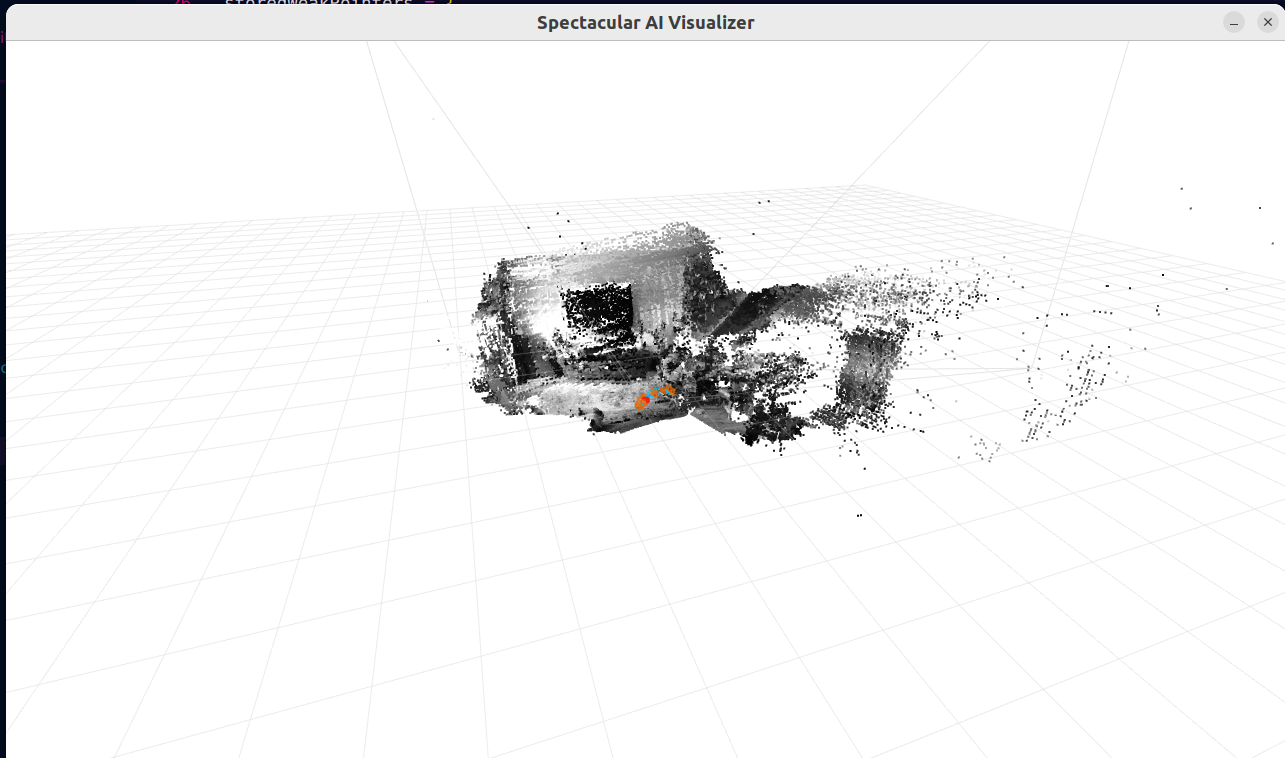
\includegraphics[width=150mm, keepaspectratio]{figures/spectacular_ai_mapping_visu.png}
	\caption{Mapping with Spectacular AI}
	\label{fig:SPAI_mapping}
\end{figure}

\begin{figure}[htbp]
	\centering
	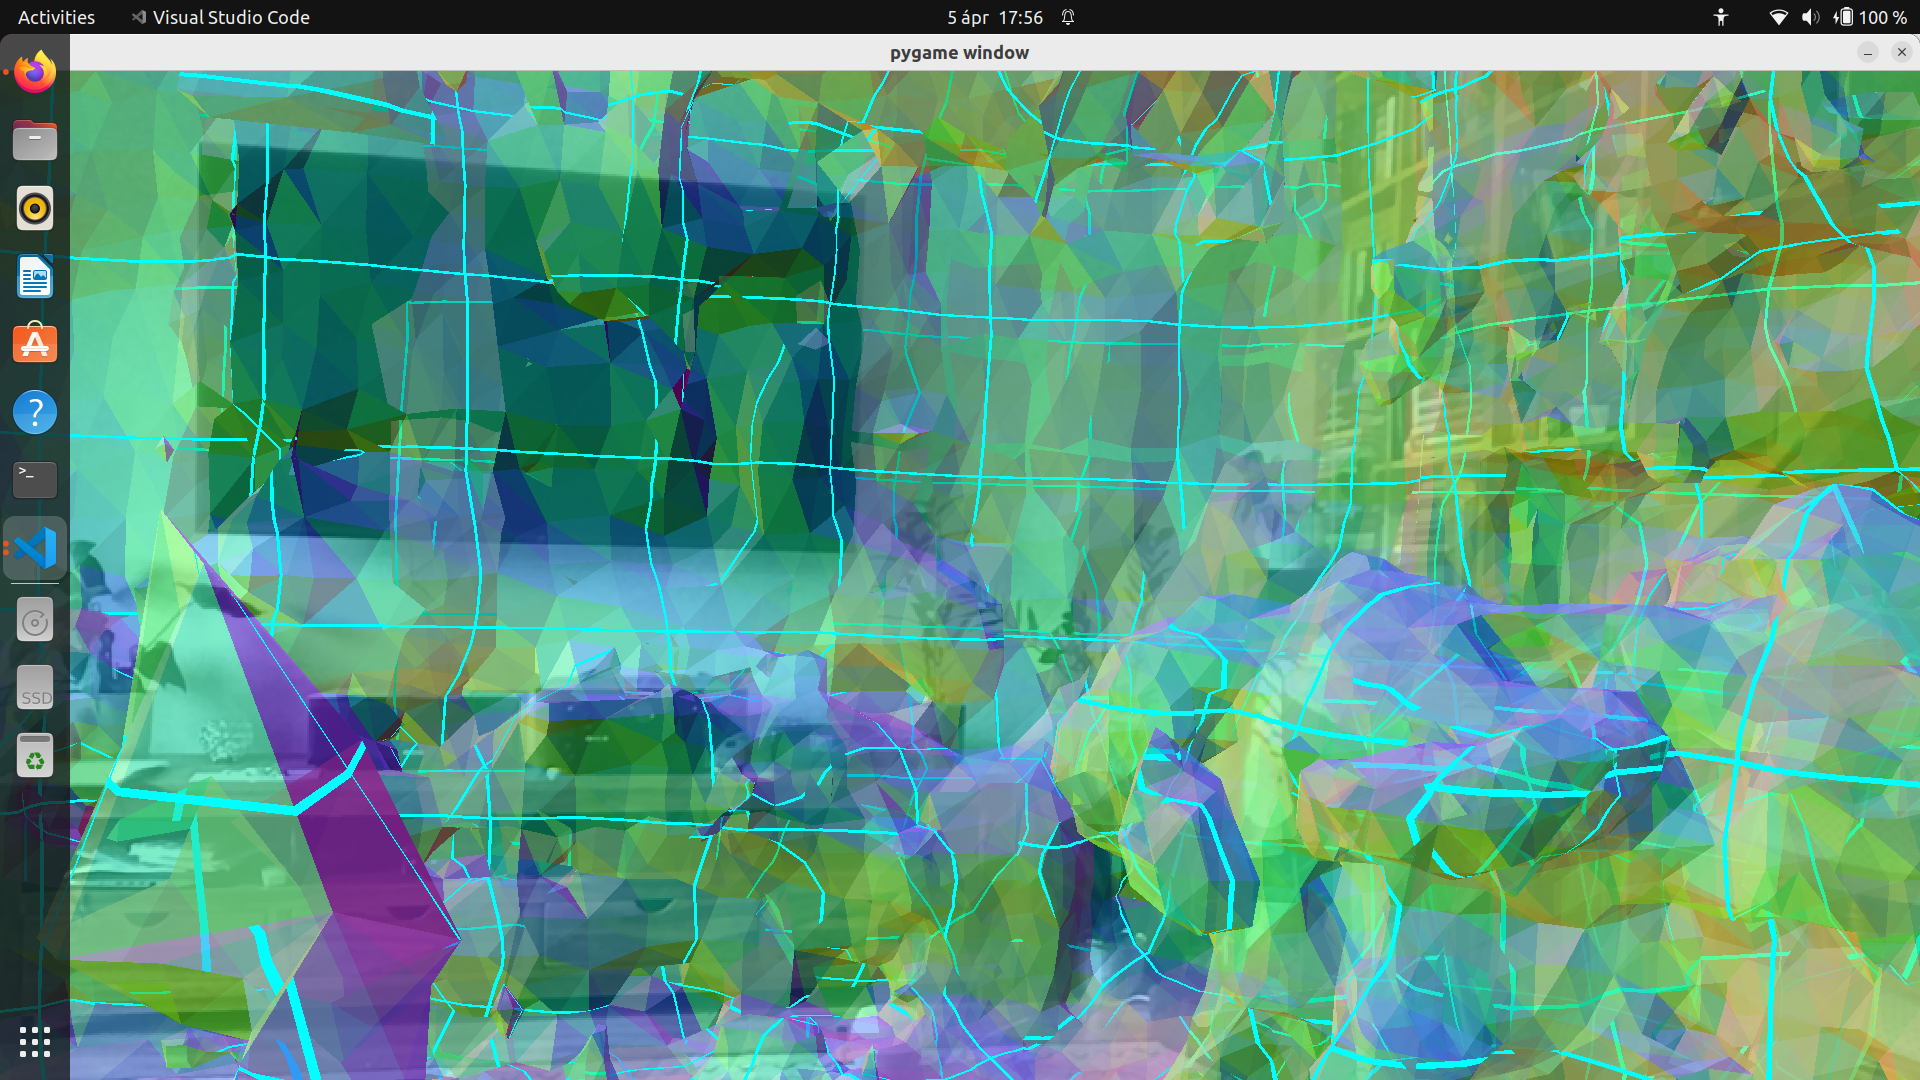
\includegraphics[width=67mm, keepaspectratio]{figures/spectacular_ai_mapping_ar_mesh1.png}\hspace{1cm}
	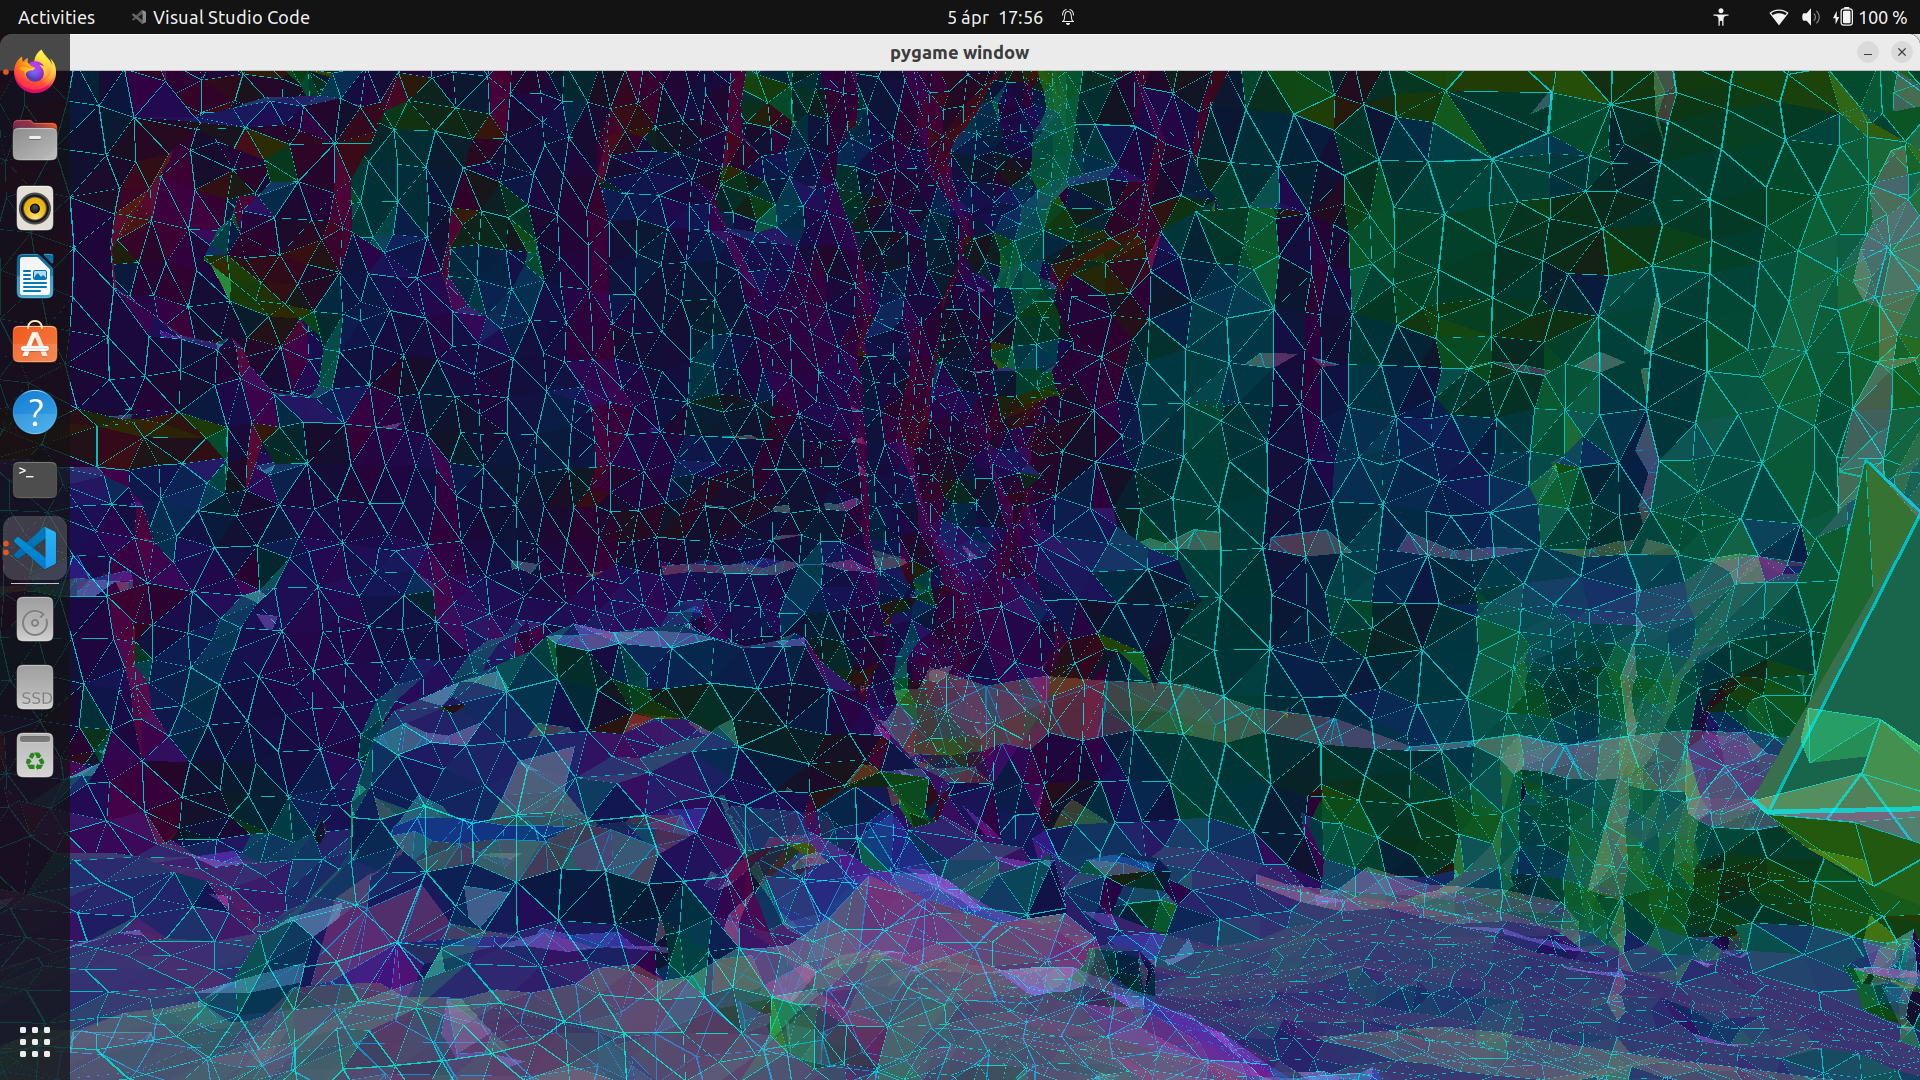
\includegraphics[width=67mm, keepaspectratio]{figures/spectacular_ai_mapping_ar_mesh2.png}\\\vspace{5mm}
	\caption{AR mesh mapping with Spectacular AI}
    \label{fig:SPAI_mesh_mapping}
\end{figure}

\begin{figure}[htbp]
	\centering
	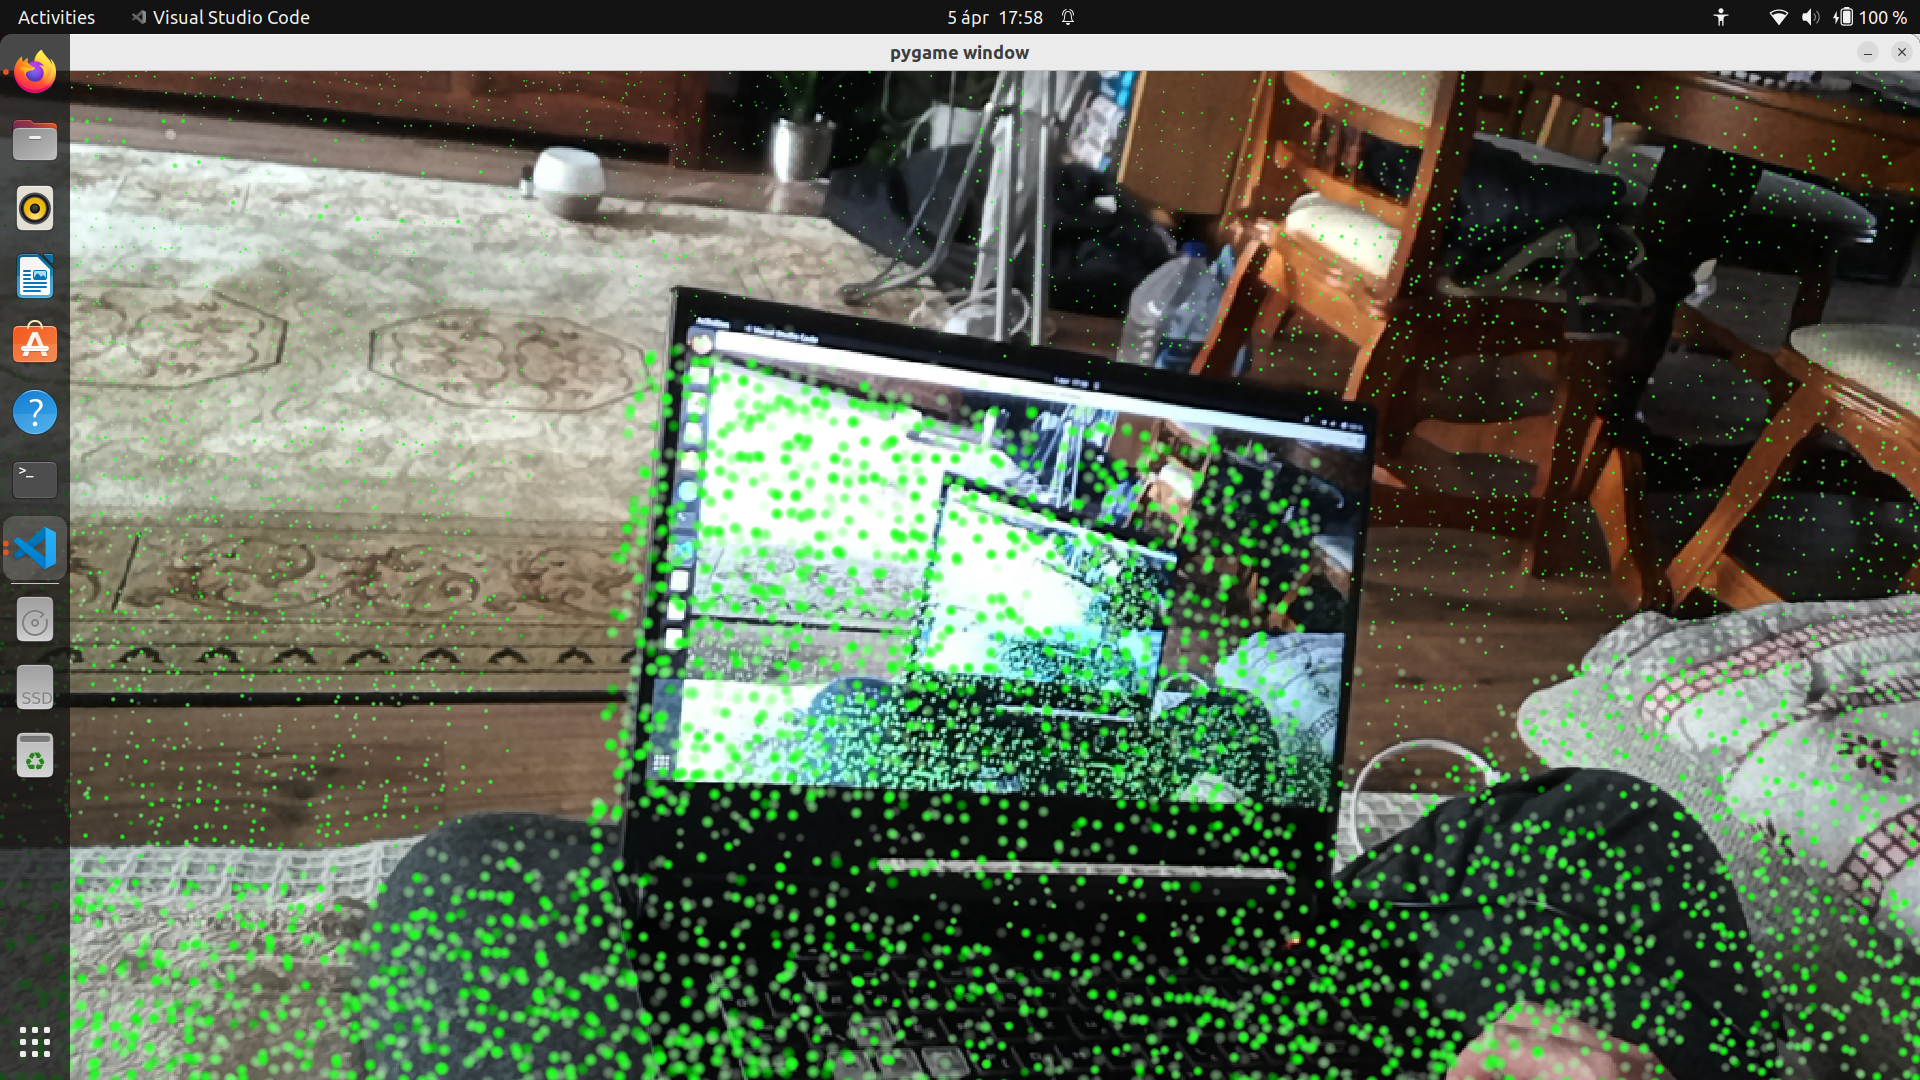
\includegraphics[width=67mm, keepaspectratio]{figures/spectacular_ai_mapping_ar_pc1.png}\hspace{1cm}
	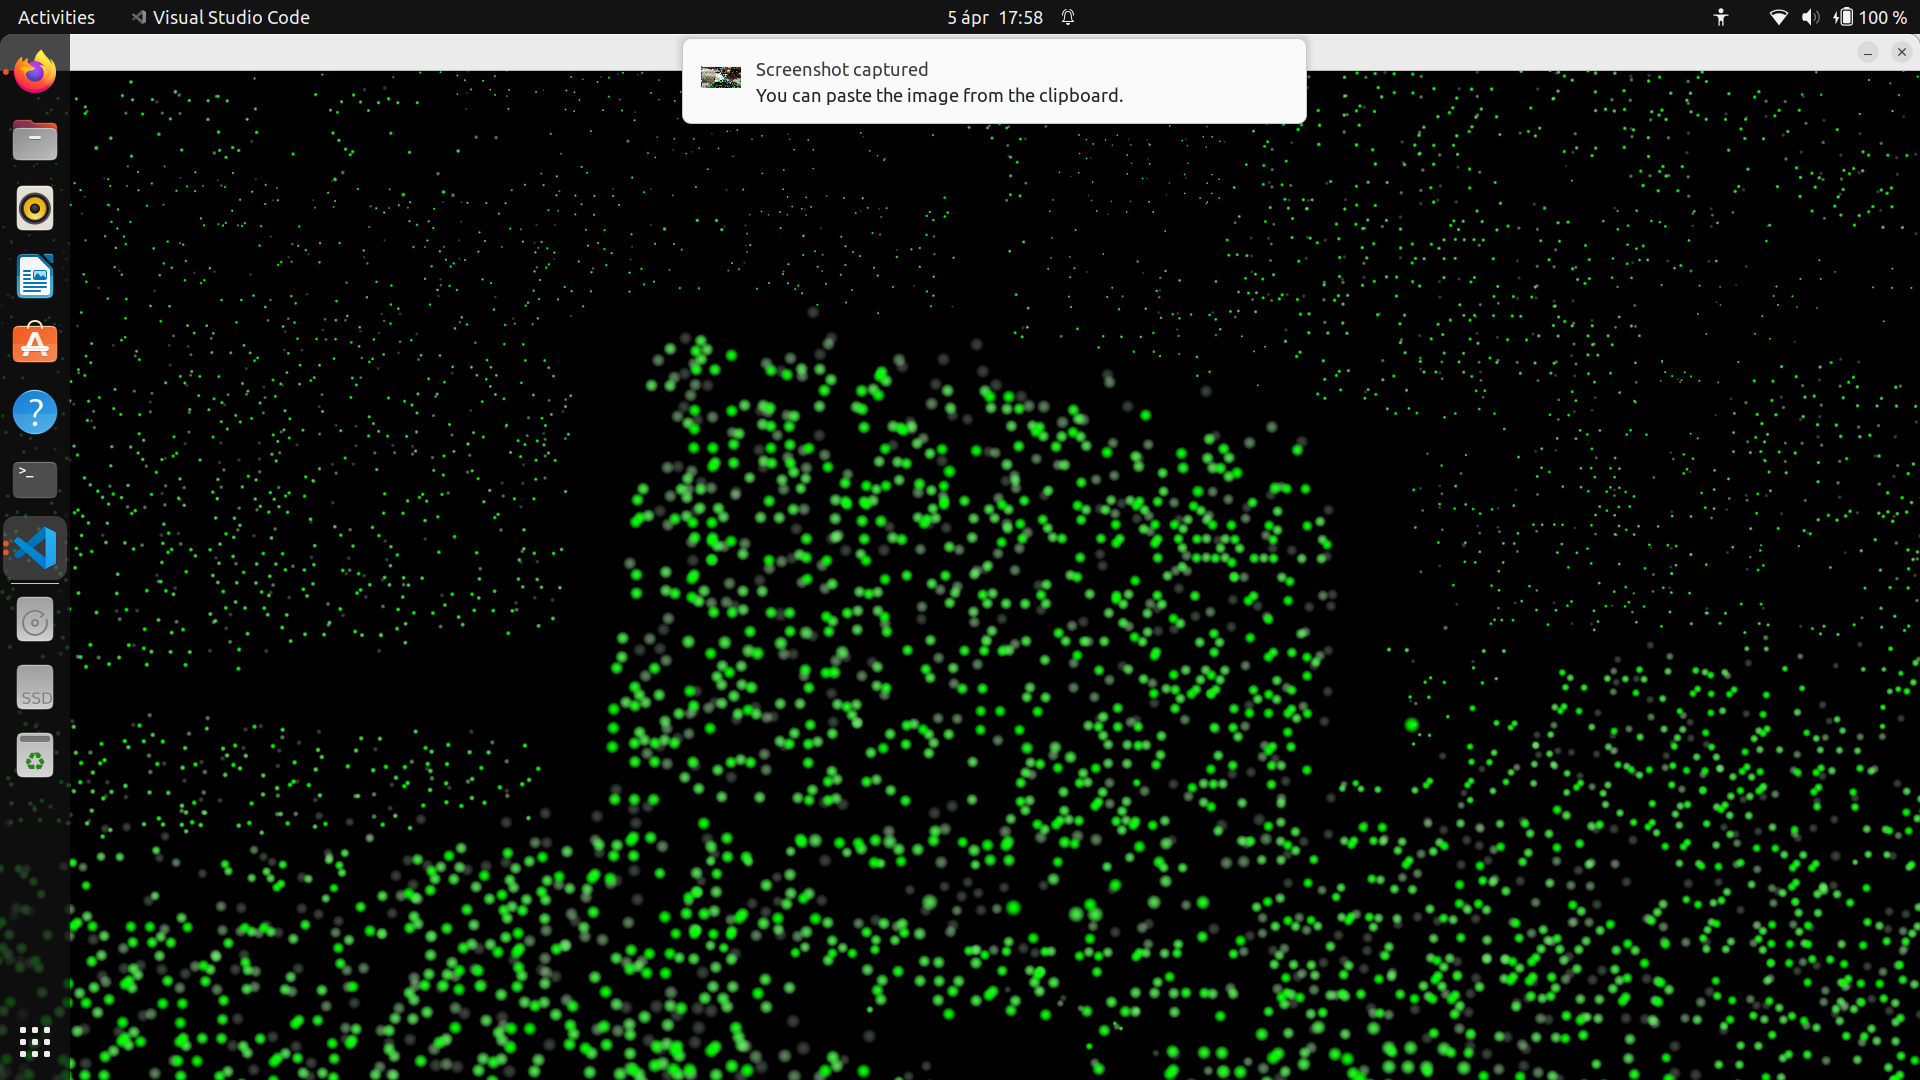
\includegraphics[width=67mm, keepaspectratio]{figures/spectacular_ai_mapping_ar_pc2.png}\\\vspace{5mm}
	\caption{AR point cloud mapping with Spectacular AI}
    \label{fig:SPAI_point_cloud_mapping}
\end{figure}

\begin{figure}[htbp]
	\centering
	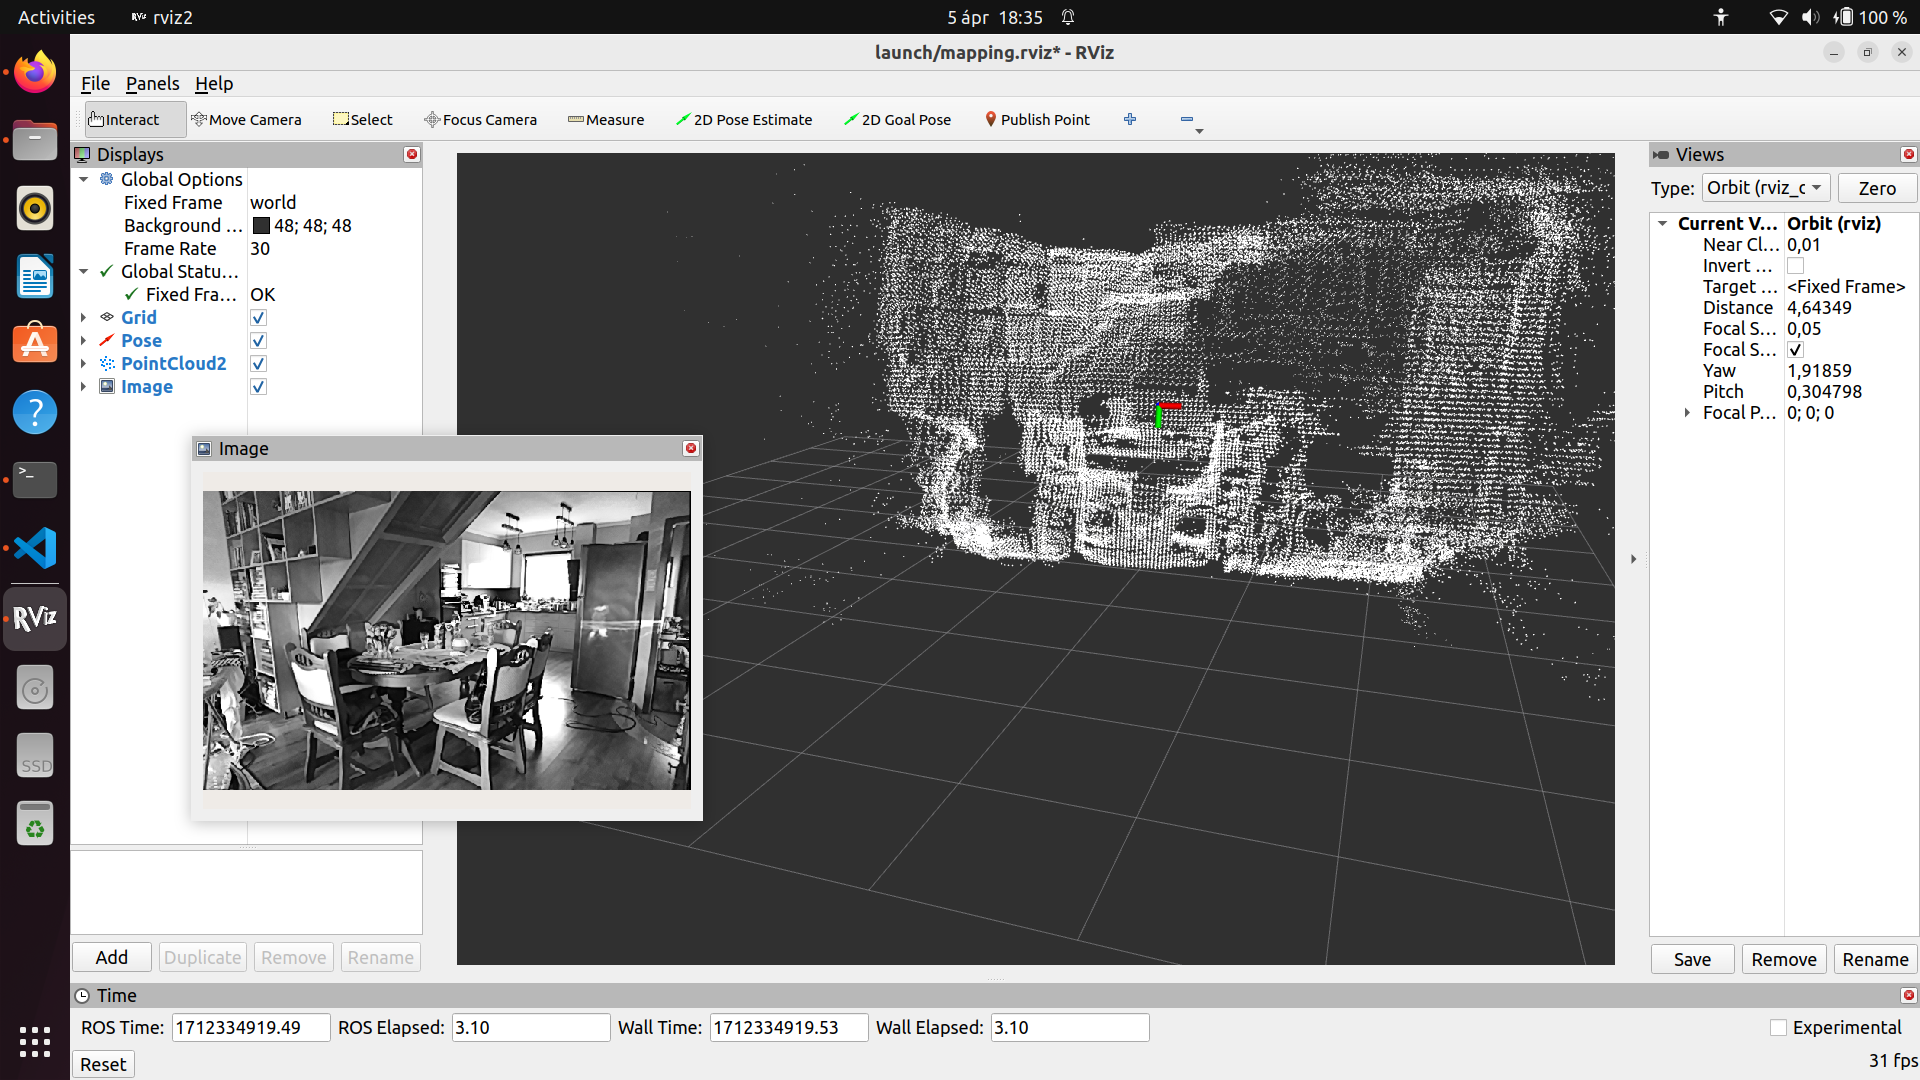
\includegraphics[width=150mm, keepaspectratio]{figures/spectacular_ai_mapping_ros2.png}
	\caption{ROS2 mapping with Spectacular AI}
	\label{fig:SPAI_ros_mapping}
\end{figure}

As we can see, the Spectacular AI SDK works really well with the OAK camera. During the testing of the examples, I could not experience any major latencies so we can safely say that it works in real time.

I saved the most exciting example for the last one of each. As I said earlier, the camera contains a VPU (Intel Movidius Myriad X\footnote{\url{https://www.intel.com/content/www/us/en/products/sku/204770/intel-movidius-myriad-x-vision-processing-unit-0gb/specifications.html}}) which can run neural network models. We do not have to make any post-processing or post-detecting with neural networks because it can be ran on the camera itself. Thanks to the stereo cameras and the VPU, the OAK-D is able to detect objects and calculate their location on the fly. To select what type of objects we want to detect, we have to modify the example code (we only have to modify one list). As we can see on Figure~\ref{fig:SPAI_depthai}, I customised the code to detect potted plants in the living room. Due to inadequate lighting the detections did not perform 100\% but they are acceptable. Moreover, I measured the positions of the plants myself and I can safely say that the camera calculated the distances really accurately.

\begin{figure}[H]
	\centering
	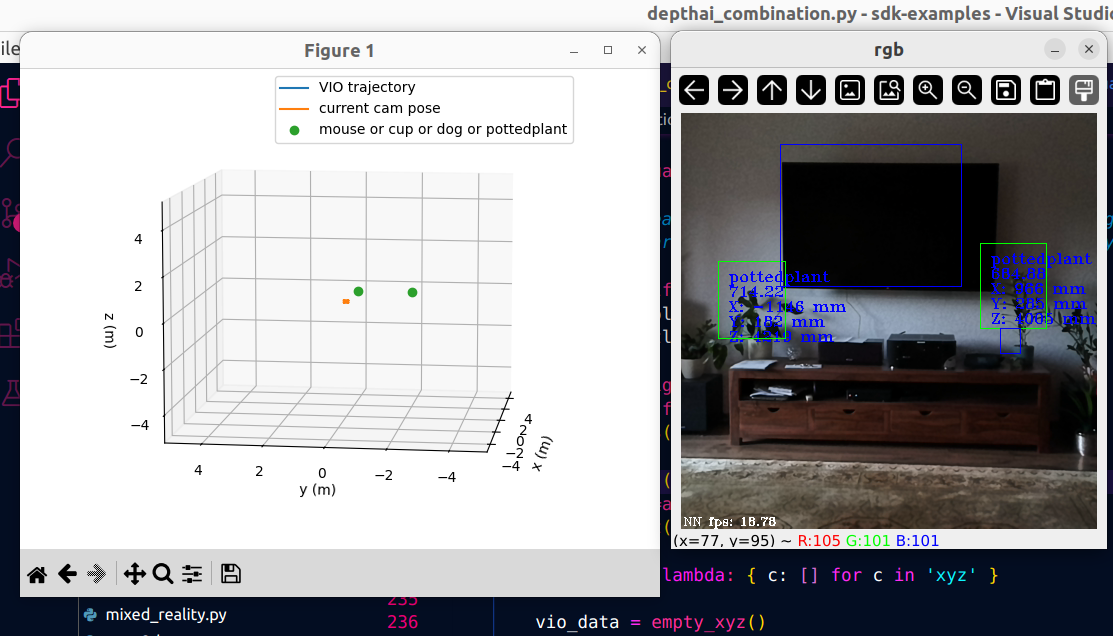
\includegraphics[width=150mm, keepaspectratio]{figures/spectacular_ai_depthai_combination.png}
	\caption{Spectacular AI's object detection and position calculation}
	\label{fig:SPAI_depthai}
\end{figure}

\GS{describe here that if we can track the camera pose in the room using SPAI and we can detect objects with depth in 3D on any camera image, that means we can detect the 3D position of objects within the room! This will be important for the mapping.}

\section{Experimenting with a custom person detector}

It was one of our goals to detect persons with the camera and make the robot follow or avoid them while mapping. For that purpose we first tried out the Spectacular AI's example on the robot's camera but we soon realized that the position of it is not ideal for detecting objects. Due to the platform above the robot it limits the FOV (Field of View) of the camera so much that if we stood 2-3 meters away from the robot only our legs were visible, thus the detection was not working. Our solution for this problem was to put the camera right at the front of the platform with some plasticine and it caused the FOV to be increased. The detection of my advisor with the camera at front can be seen on Figure \ref{fig:person_detection_camera_at_front_nokia} (the other detected person is a woman on a poster).

\begin{figure}[htbp]
    \centering
    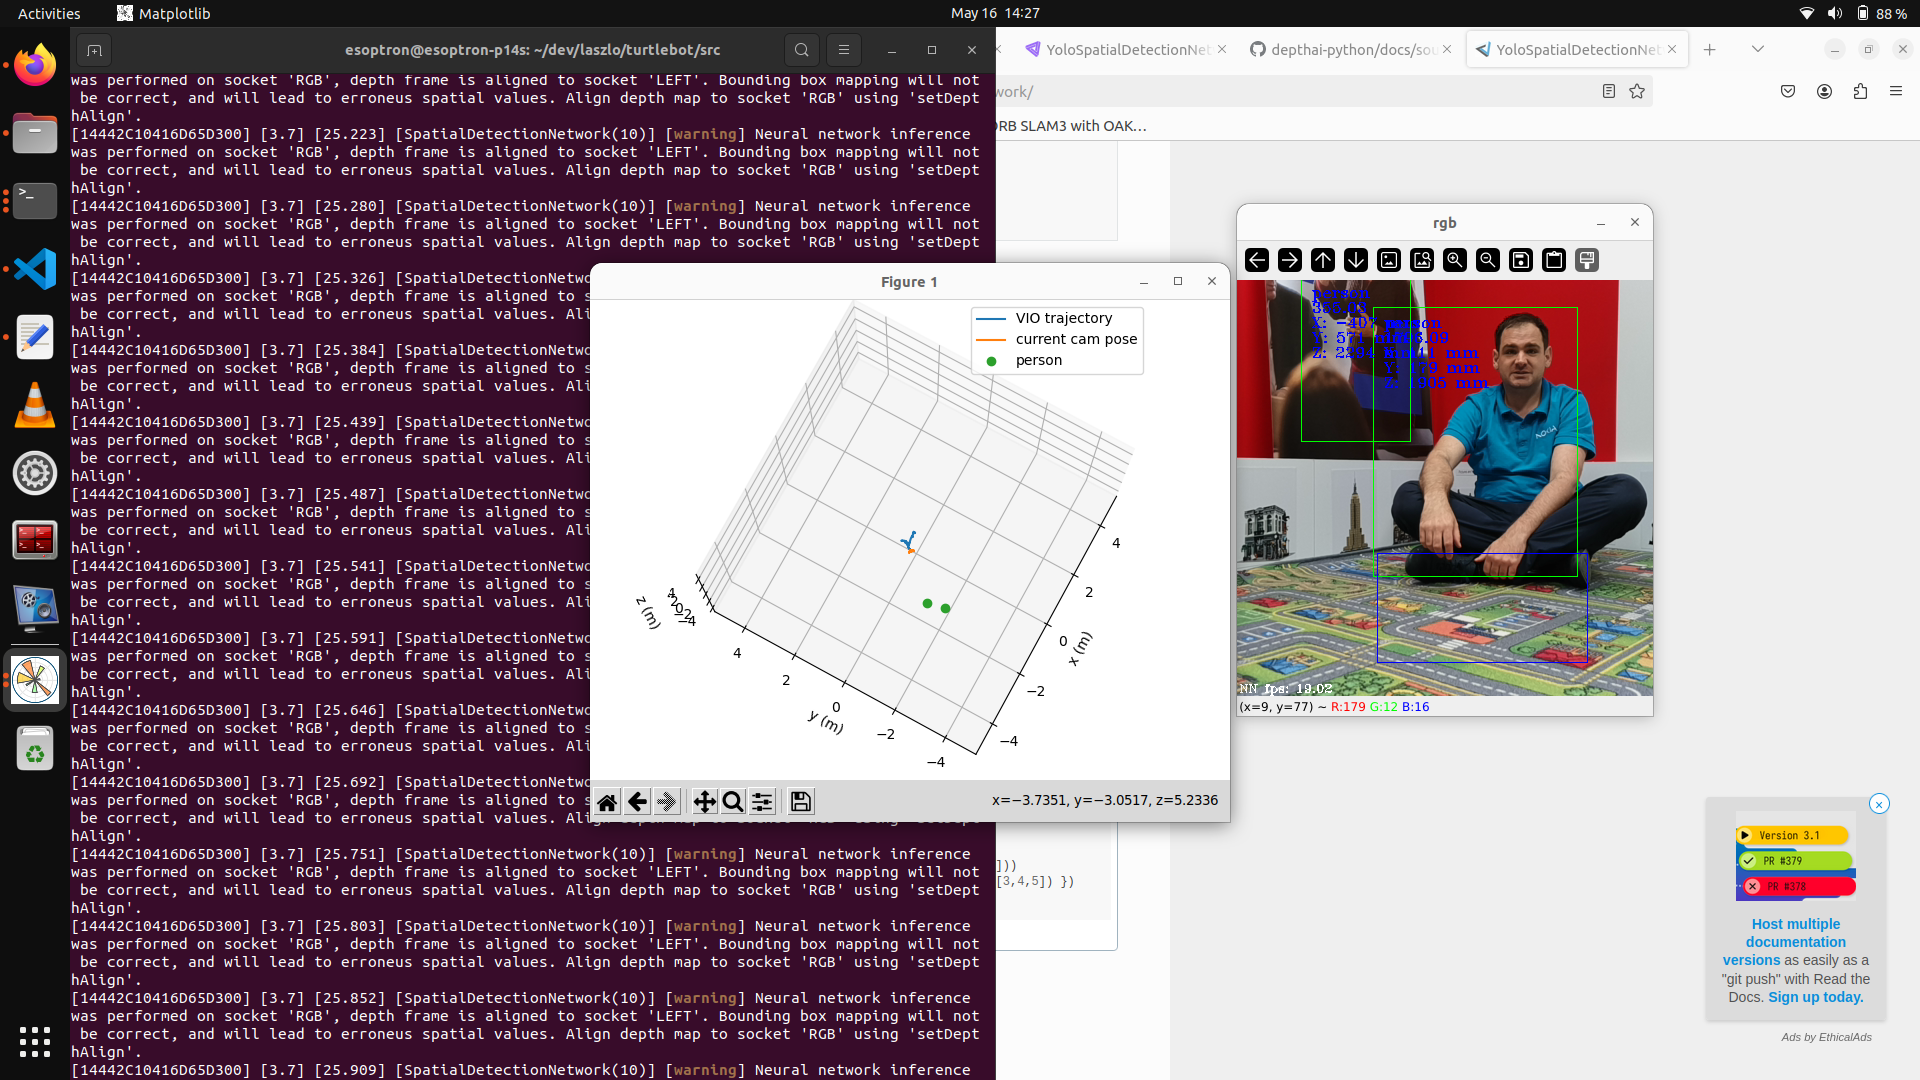
\includegraphics[width=150mm, keepaspectratio]{figures/person_detection_camera_at_front_nokia.png}
    \caption{Person detection with the camera at front at Nokia Bell Labs}
    \label{fig:person_detection_camera_at_front_nokia}
\end{figure}

After we experimented with the FOV and the example detection script I created a custom script based on the example which uses the camera to detect persons and publish their location in world coordinates on a ROS topic (the code can be examined at \ref{custom_person_detector}). The base example and my custom person detector froze after some detections with an error indicating that the IMU buffer size is exceeded. It happens because the IMU sends data too rapidly, the configuration of the \verb|SpatialLocationCalculator| node uses a buffer that is too small for storing that much data and, on top of that, it does not flush the buffer frequently enough. That buffer cannot be extended or flushed because it is fixed in the aforementioned node. In conclusion, we could not implement a stable person detection using this camera due to its previously stated limitations.
